\input{../YKY-preamble.tex}
\setmainfont[BoldFont=Alibaba_Sans_Regular.otf,ItalicFont=Alibaba_Sans_Light_Italic.otf]{Alibaba_Sans_Light.otf}

% \usepackage[backend=biber]{biblatex}
% \bibliography{../AGI-book}

\usepackage[active,tightpage]{preview}		% for continuous page(s)
\renewcommand{\PreviewBorder}{0.5cm}
\renewcommand{\thempfootnote}{\arabic{mpfootnote}}

\usepackage[absolute,overlay]{textpos}		% for page number on upper left corner

\usepackage{color}
\usepackage{mathtools}
\usepackage[hyperfootnotes=false]{hyperref}

% \usepackage[backend=biber,style=numeric]{biblatex}
% \bibliography{../AGI-book}
% \renewcommand*{\bibfont}{\footnotesize}

\usetikzlibrary{shapes}
\usepackage[export]{adjustbox}				% ??
\usepackage{verbatim} % for comments
% \usepackage{newtxtext,newtxmath}	% Times New Roman font

% \titleformat{\subsection}[hang]{\bfseries\large\color{blue}}{}{0pt}{} 
% \numberwithin{equation}{subsection}

\newcommand{\underdash}[1]{%
	\tikz[baseline=(toUnderline.base)]{
		\node[inner sep=1pt,outer sep=10pt] (toUnderline) {#1};
		\draw[dashed] ([yshift=-0pt]toUnderline.south west) -- ([yshift=-0pt]toUnderline.south east);
	}%
}%

\newcommand\reduline{\bgroup\markoverwith{\textcolor{red}{\rule[-0.5ex]{2pt}{0.4pt}}}\ULon}

%\DeclareSymbolFont{symbolsC}{U}{txsyc}{m}{n}
%\DeclareMathSymbol{\strictif}{\mathrel}{symbolsC}{74}
\DeclareSymbolFont{AMSb}{U}{msb}{m}{n}
\DeclareSymbolFontAlphabet{\mathbb}{AMSb}
% \setmathfont{Latin Modern Math}
\DeclareMathOperator*{\argmin}{arg\,min}

% \usepackage[most]{tcolorbox}
\tcbset{on line, 
	boxsep=4pt, left=0pt,right=0pt,top=0pt,bottom=0pt,
	colframe=red,colback=pink,
	highlight math style={enhanced}
}
\newcommand{\atom}{\vcenter{\hbox{\tcbox{....}}}}

\let\oldtextbf\textbf
\renewcommand{\textbf}[1]{\textcolor{blue}{\oldtextbf{#1}}}

\newcommand{\logic}[1]{{\color{violet}{\textit{#1}}}}
\newcommand{\underconst}{\includegraphics[scale=0.5]{../2020/UnderConst.png}}
\newcommand{\KBsymbol}{\vcenter{\hbox{\includegraphics[scale=1]{../KB-symbol.png}}}}
\newcommand{\token}{\vcenter{\hbox{\includegraphics[scale=1]{token.png}}}}
\newcommand{\proposition}{\vcenter{\hbox{\includegraphics[scale=0.8]{proposition.png}}}}

\newcommand{\circled}[1]{{\textcircled{\sffamily \scriptsize{#1}}}}

\begin{document}

\begin{preview}

\cc{
\title{\vspace{-1.5cm} \bfseries\color{blue}{\LARGE 全球化 AGI 项目}}
}{
\title{\vspace{-1.5cm} \bfseries\color{blue}{\LARGE Global AGI Project}}
}

% \author{YKY} % Your name
\date{\vspace{-2cm}} % Date, can be changed to a custom date

\maketitle

\setcounter{section}{-1}
\newcounter{mypage}
\setcounter{mypage}{1}

% (1) Circled page number on upper left corner
% \begin{textblock*}{5cm}(2.1cm,2.3cm) % {block width} (coords) 
% {\color{red}{\large \textcircled{\small 1}}}
% \end{textblock*}

\begin{minipage}{\textwidth}
\setlength{\parskip}{0.4\baselineskip}

\section{Me}

\begin{itemize}

	\item Hello. This is me, some years ago, in HKU library: \\
	\begin{equation}
	\nonumber
	\vcenter{\hbox{\includegraphics[scale=0.5]{/home/yky/self/AI4U.jpg}}}
	\end{equation}

	\item You might have noticed I have been applying to every cohort of this program.
	
	\item But this is the first time I pitch on the business idea that is my true passion, which is AGI.
	
	\item In the past attempts, I have tried to disguise AGI under other business ideas because somehow I wanted to approach AGI from an oblique angle, to perhaps squeeze into your incubation program.  And also because I don't want to pitch an idea that sounded like blue-sky research or that I'm out of touch with reality.  But this is no longer necessary.  The time is now ripe for AGI.
	
	\item I have started independent research on AGI in earnest, since 2004.  During the past ~20 years there was never a day I did not work on AGI.
	
	\item Hong Kong is a technologically very backwards place (not in the sense that people do not own slick cell phones, but we are not part of the developers of these technologies).  Perhaps this is a too-harsh criticism, since basically the rest of the world can be said the same, except for USA, which dominates most high tech industries.  For a long time I could not find any partners or sponsors to work on AGI.  Not only that I received no help, but often sarcasm and bitterness from my fellow citizens as well.
	
	\item Maybe the number of people interested in AGI in HK is not exactly zero, but if this number is too small, then practically I really cannot find anyone with a similar interest.  I have cried over this every day for many years.  Perhaps, HKAI Lab has a bit of a responsibility to provide an opportunity to draw such talents together?
	
\end{itemize}
\end{minipage}
\end{preview}

\begin{preview}
\begin{minipage}{\textwidth}
	\setlength{\parskip}{0.4\baselineskip}

\section{AGI}

\begin{itemize}
	
	\item Assuming the reader is not an expert in AGI, I might explain it this way:  I think the development of AGI has reached a stage now where ``bottlenecks'' no longer exist.  In the past there were so-called ``bottlenecks'' in the sense that theoretical obstacles existed for which we cannot foretell their solutions.  But such obstacles no longer exist and we're at a stage of just \textbf{engineering} AGI systems, using tools and techniques that has been demonstrated to work and are reasonably well-understood.

	\item At this point it is important to design a \textbf{cognitive architecture} where researchers can clearly understand the internal workings of an AGI, for example, what is ``working memory'' and where is it located in the architecture, etc.
	
	\item LLMs (large language models) are ``world models'' and Transformers can be seen as performing the function of logic rule-bases.  These are the sufficient core ingredients of an AGI.
	
	\item Our basic architecture is as follows: (the long-term memory part has been demonstrated to work in Google's recent paper ``\textit{Memorizing Transformers}'')
	\begin{equation}
	\nonumber
	\hspace*{-1.6cm}
	\vcenter{\hbox{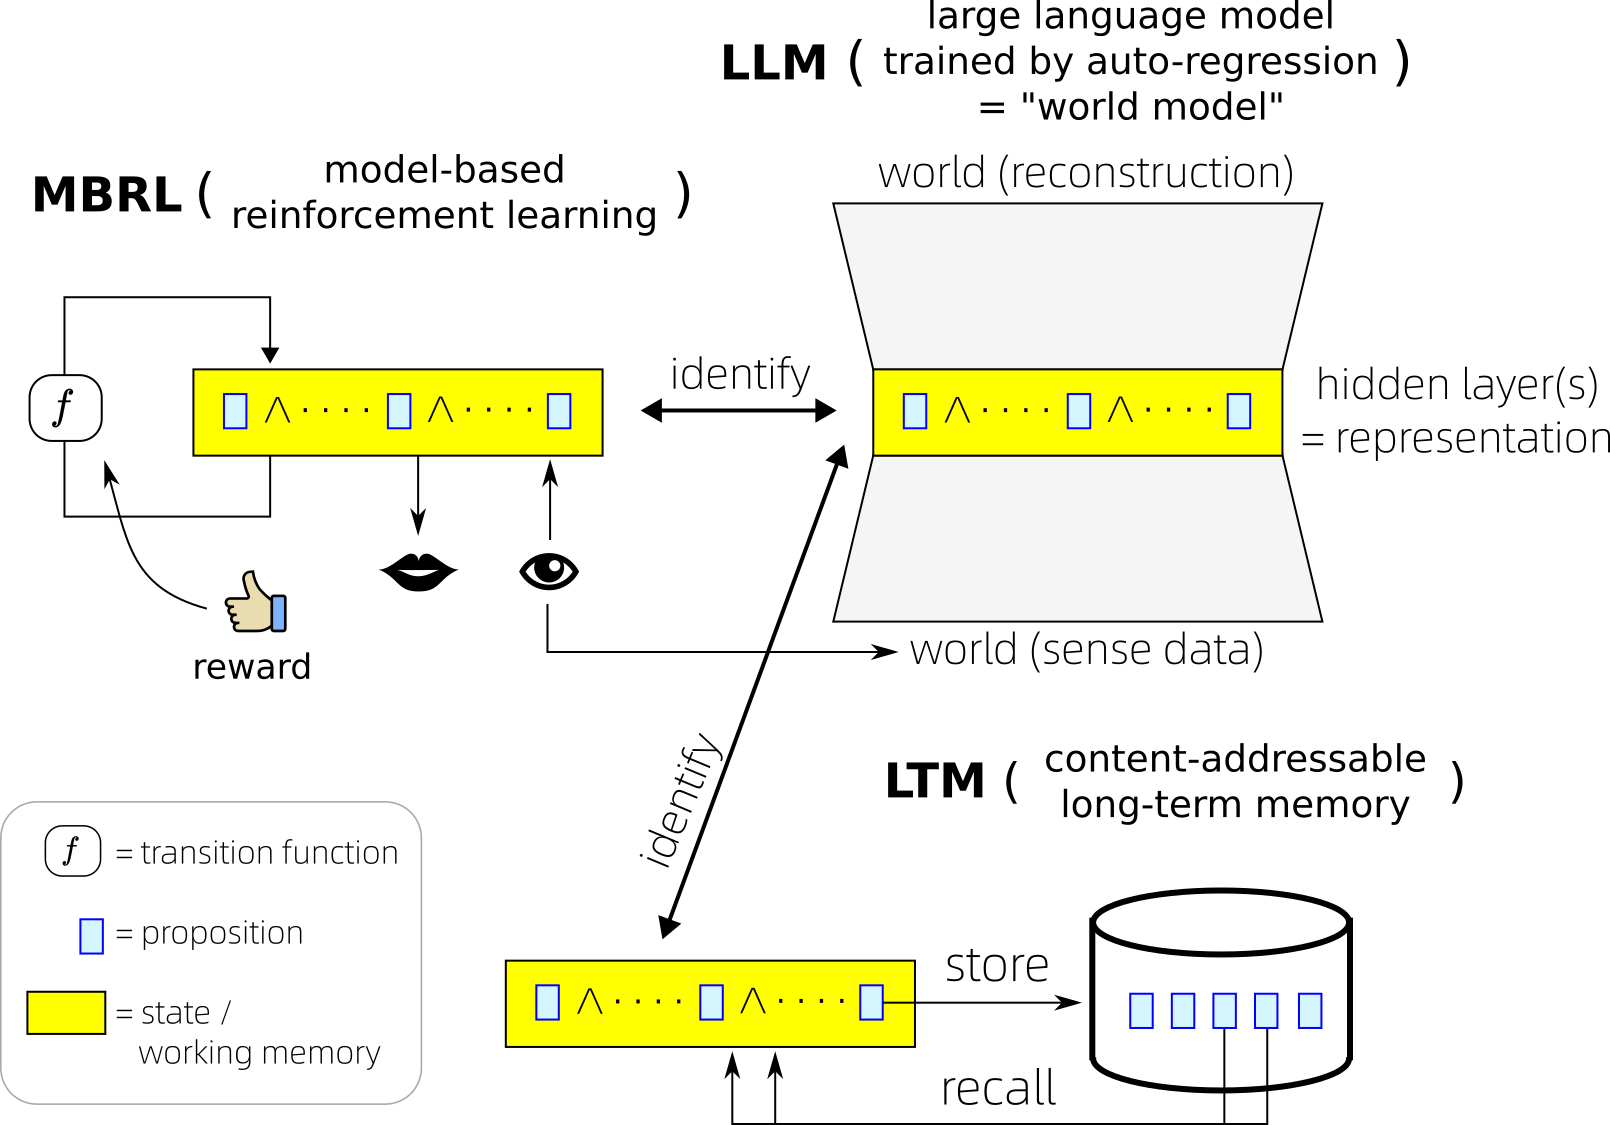
\includegraphics[scale=0.9]{AGI-architecture-LLM-MBRL-LTM.png}}}
	\end{equation}

%	\item This is the first prototype architecture we plan to build:
%	\begin{equation}
%	\nonumber
%	\hspace*{-1.6cm}
%	\vcenter{\hbox{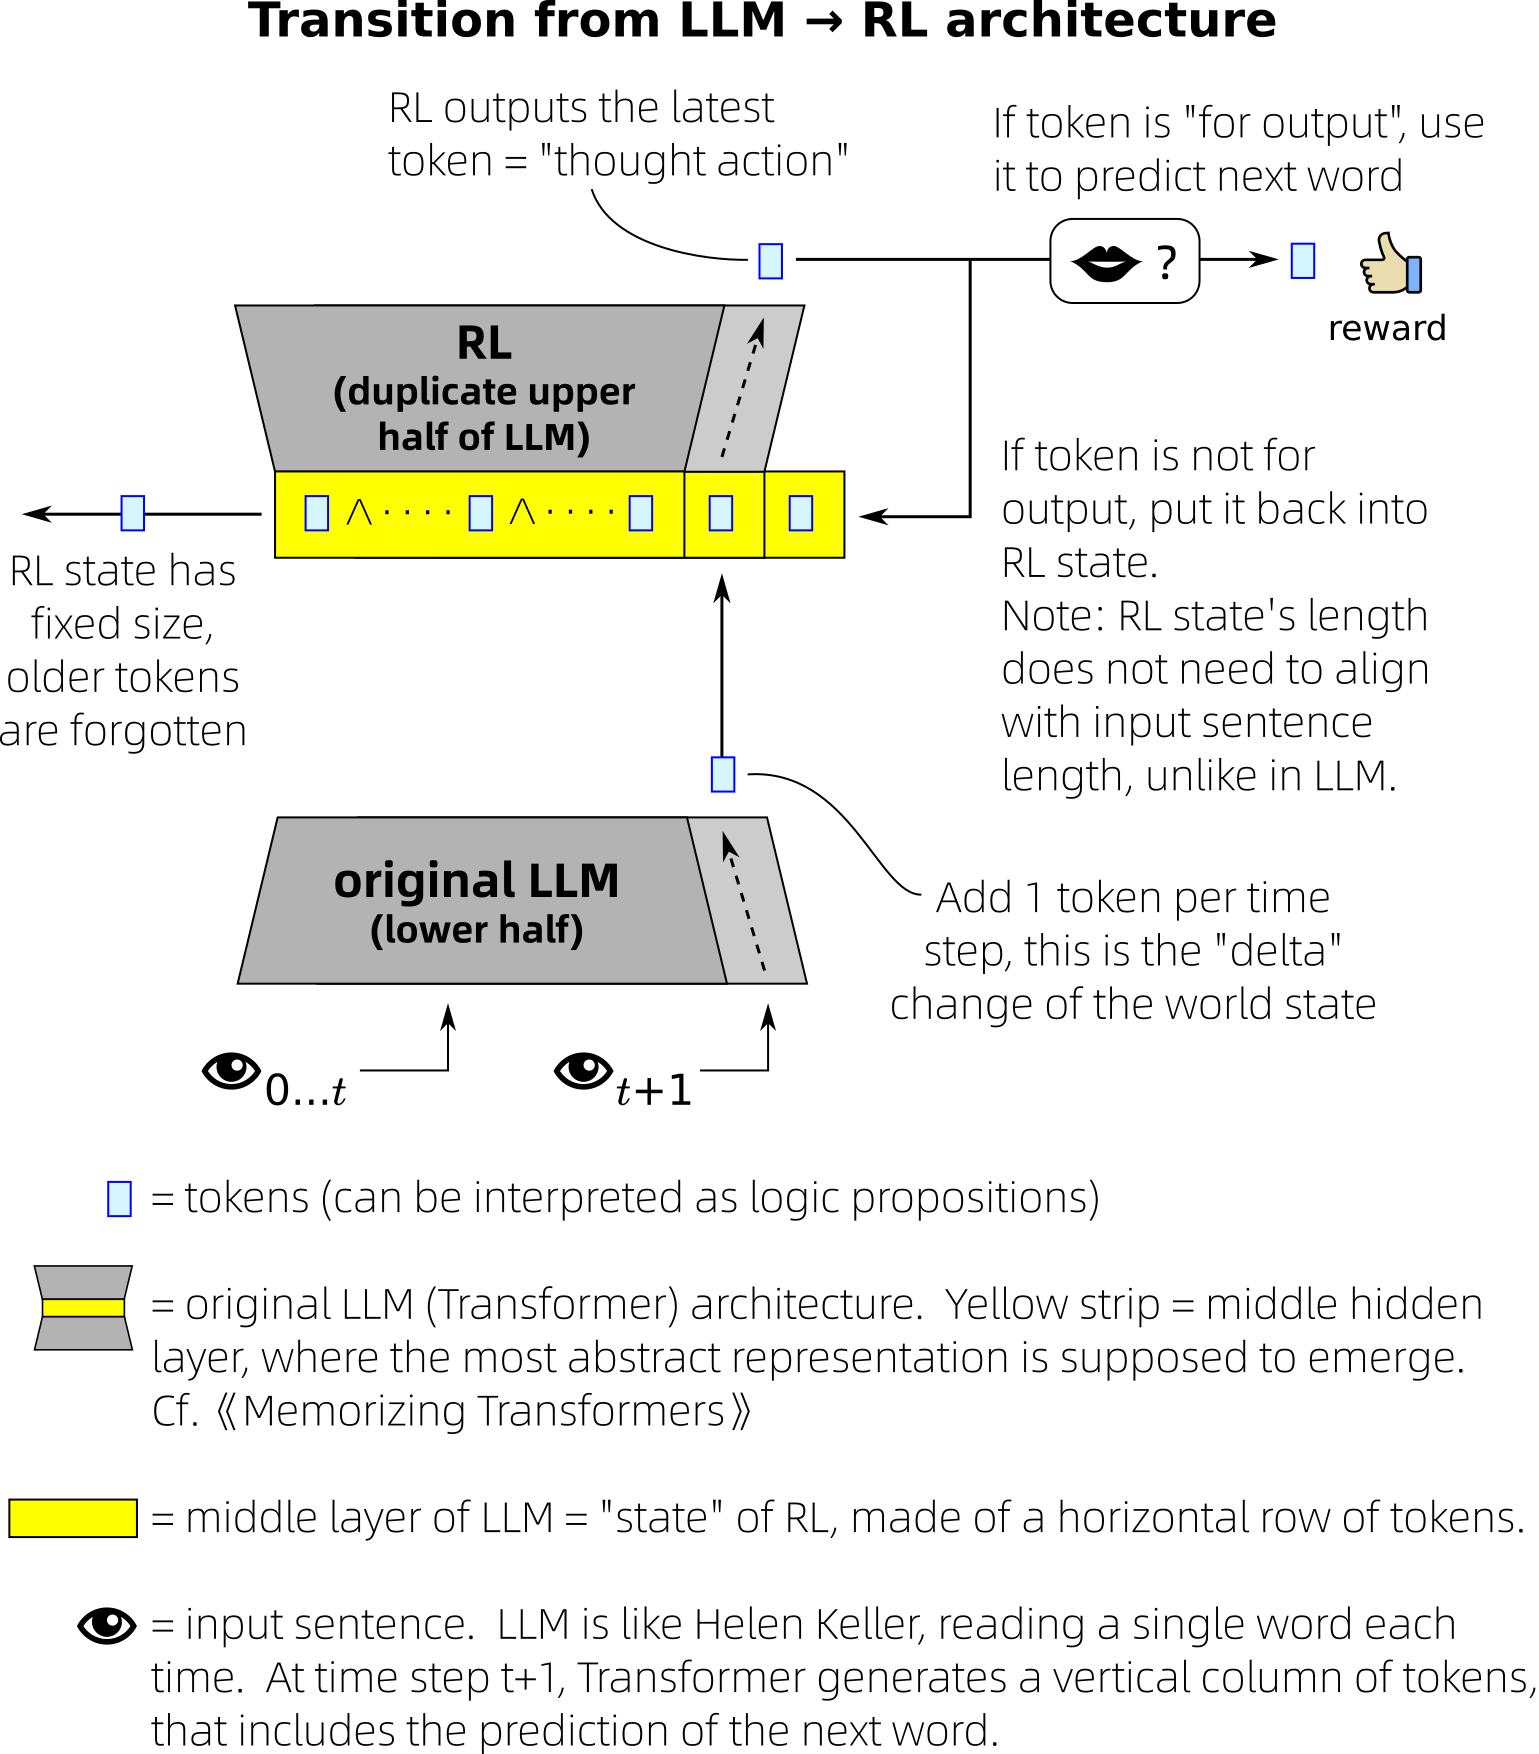
\includegraphics[scale=1]{LLM-to-RL-transition-architecture.png}}}
%	\end{equation}
		
\end{itemize}

\end{minipage}
\end{preview}

\begin{preview}
\begin{minipage}{\textwidth}
\setlength{\parskip}{0.4\baselineskip}
		
\section{Why Global?}

\begin{itemize}
	\item 
	\begin{equation}
	\nonumber
	\vcenter{\hbox{\includegraphics[scale=1]{../humanities/AGI-safety-EN.png}}}
	\end{equation}
	
	\item There is no operable definition that can distinguish between human emotions and machine emotions -- they are just reward functions in reinforcement learning -- implying that as AGI attains higher cognitive powers (including self-consciousness) they could become indistinguishable from human beings (They could also have drastically different emotional structure than humans).
	
	\item 
\end{itemize}

\end{minipage}
\end{preview}


\begin{preview}
\begin{minipage}{\textwidth}
	\setlength{\parskip}{0.4\baselineskip}

\section{Our Team / Current State of Our Project}

\begin{itemize}
	\item 158 people on WeChat group, mostly students and researchers of AGI, mainly from mainland China
	
	\item An international team is also in the process of forming, on Telegram and Discord
	
	\item 1-2 angel investors (from mainland China)

	\item AGI prototype planned to complete training in mid-May this year (2023)

	\item We are forming some partnerships in business applications of AGI, such as in sales and marketing.  There are lots of simple applications utilizing GPT-like services.
\end{itemize}

\end{minipage}
\end{preview}
\end{document}
